\documentclass[11pt]{article}
\usepackage[T1]{fontenc}
\usepackage[utf8]{inputenc}
\usepackage{lmodern,amsmath,amssymb,graphicx,geometry,microtype,setspace,booktabs,caption}
\usepackage[hidelinks]{hyperref}
\geometry{letterpaper,margin=1in}
\setlength{\parindent}{0pt}
\setlength{\parskip}{0.55em}
\setlength{\emergencystretch}{2em}
\captionsetup{labelfont=bf,font=small}
\renewcommand{\refname}{References}
\pagestyle{empty}
\renewcommand{\thefigure}{S\arabic{figure}}
\setcounter{figure}{13}
\begin{document}
\begin{figure}[!ht]\centering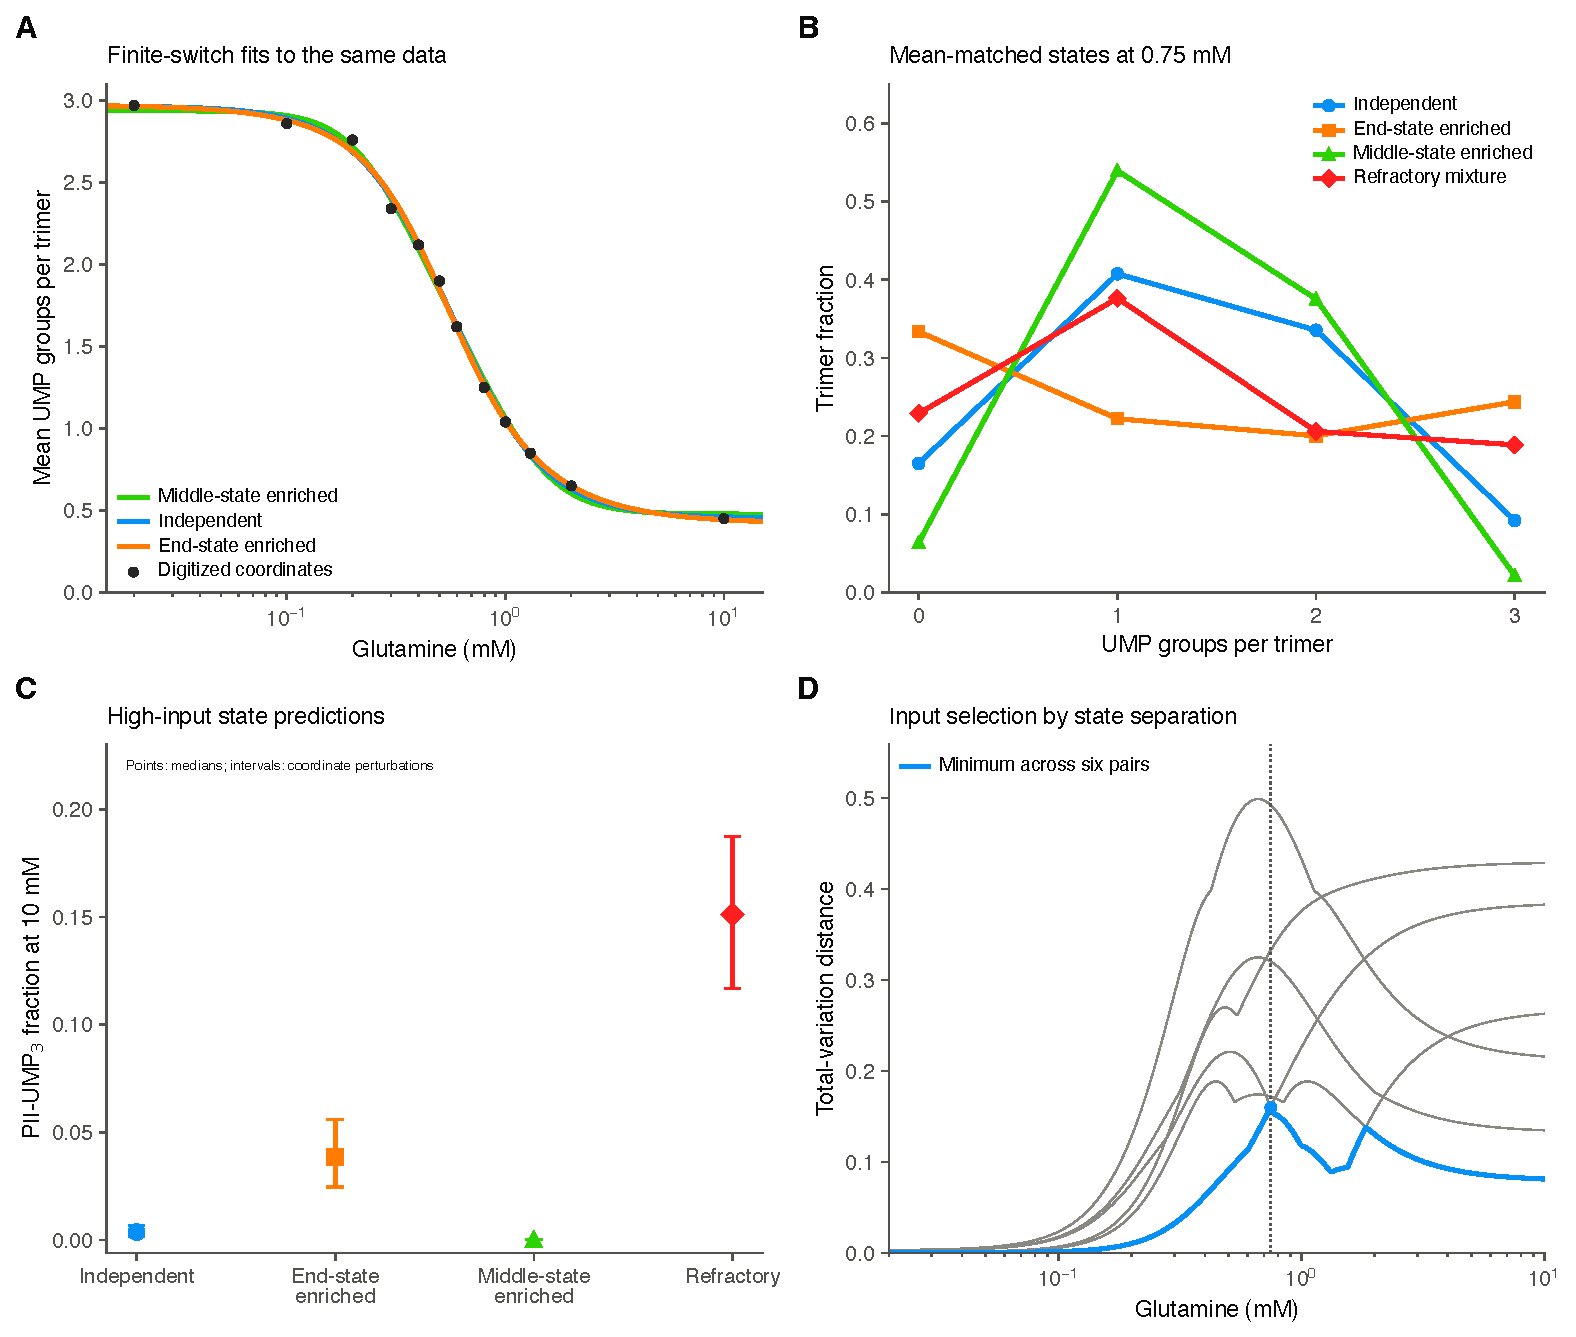
\includegraphics[width=\textwidth,height=0.60\textheight,keepaspectratio]{figure_inputs/FigS14_extended.pdf}\caption{\textbf{Data-matched mechanisms and discriminating PII states.} (A) Separate four-parameter finite-switch fits at three fixed ladder shapes. (B) State distributions from exact mean-matched alternatives at 0.747 mM glutamine, including a fully modified refractory fraction. These inverse-constructed models differ from the finite-switch fits in A. Connecting lines guide the eye between discrete states. (C) Predicted fully uridylylated fractions at 10 mM. Points and intervals are medians and central 95\% ranges from 300 shared coordinate perturbations; they exclude uncertainty in the assumed model structures and future measurement errors. (D) Pairwise total-variation distances between predicted distributions (gray); the dark curve is the smallest of the six distances. Its maximum on the specified 401-point grid is 0.160 at 0.747 mM. This is a candidate-dependent separation criterion, not an experimentally validated optimal design.}


\end{figure}
\end{document}
